定性的評価の,5段階評価項目の結果は以下の通り.
記載した箱ひげ図については,左から質問1から12の順に並んでいる.
\begin{figure}[tp]
  \centering
  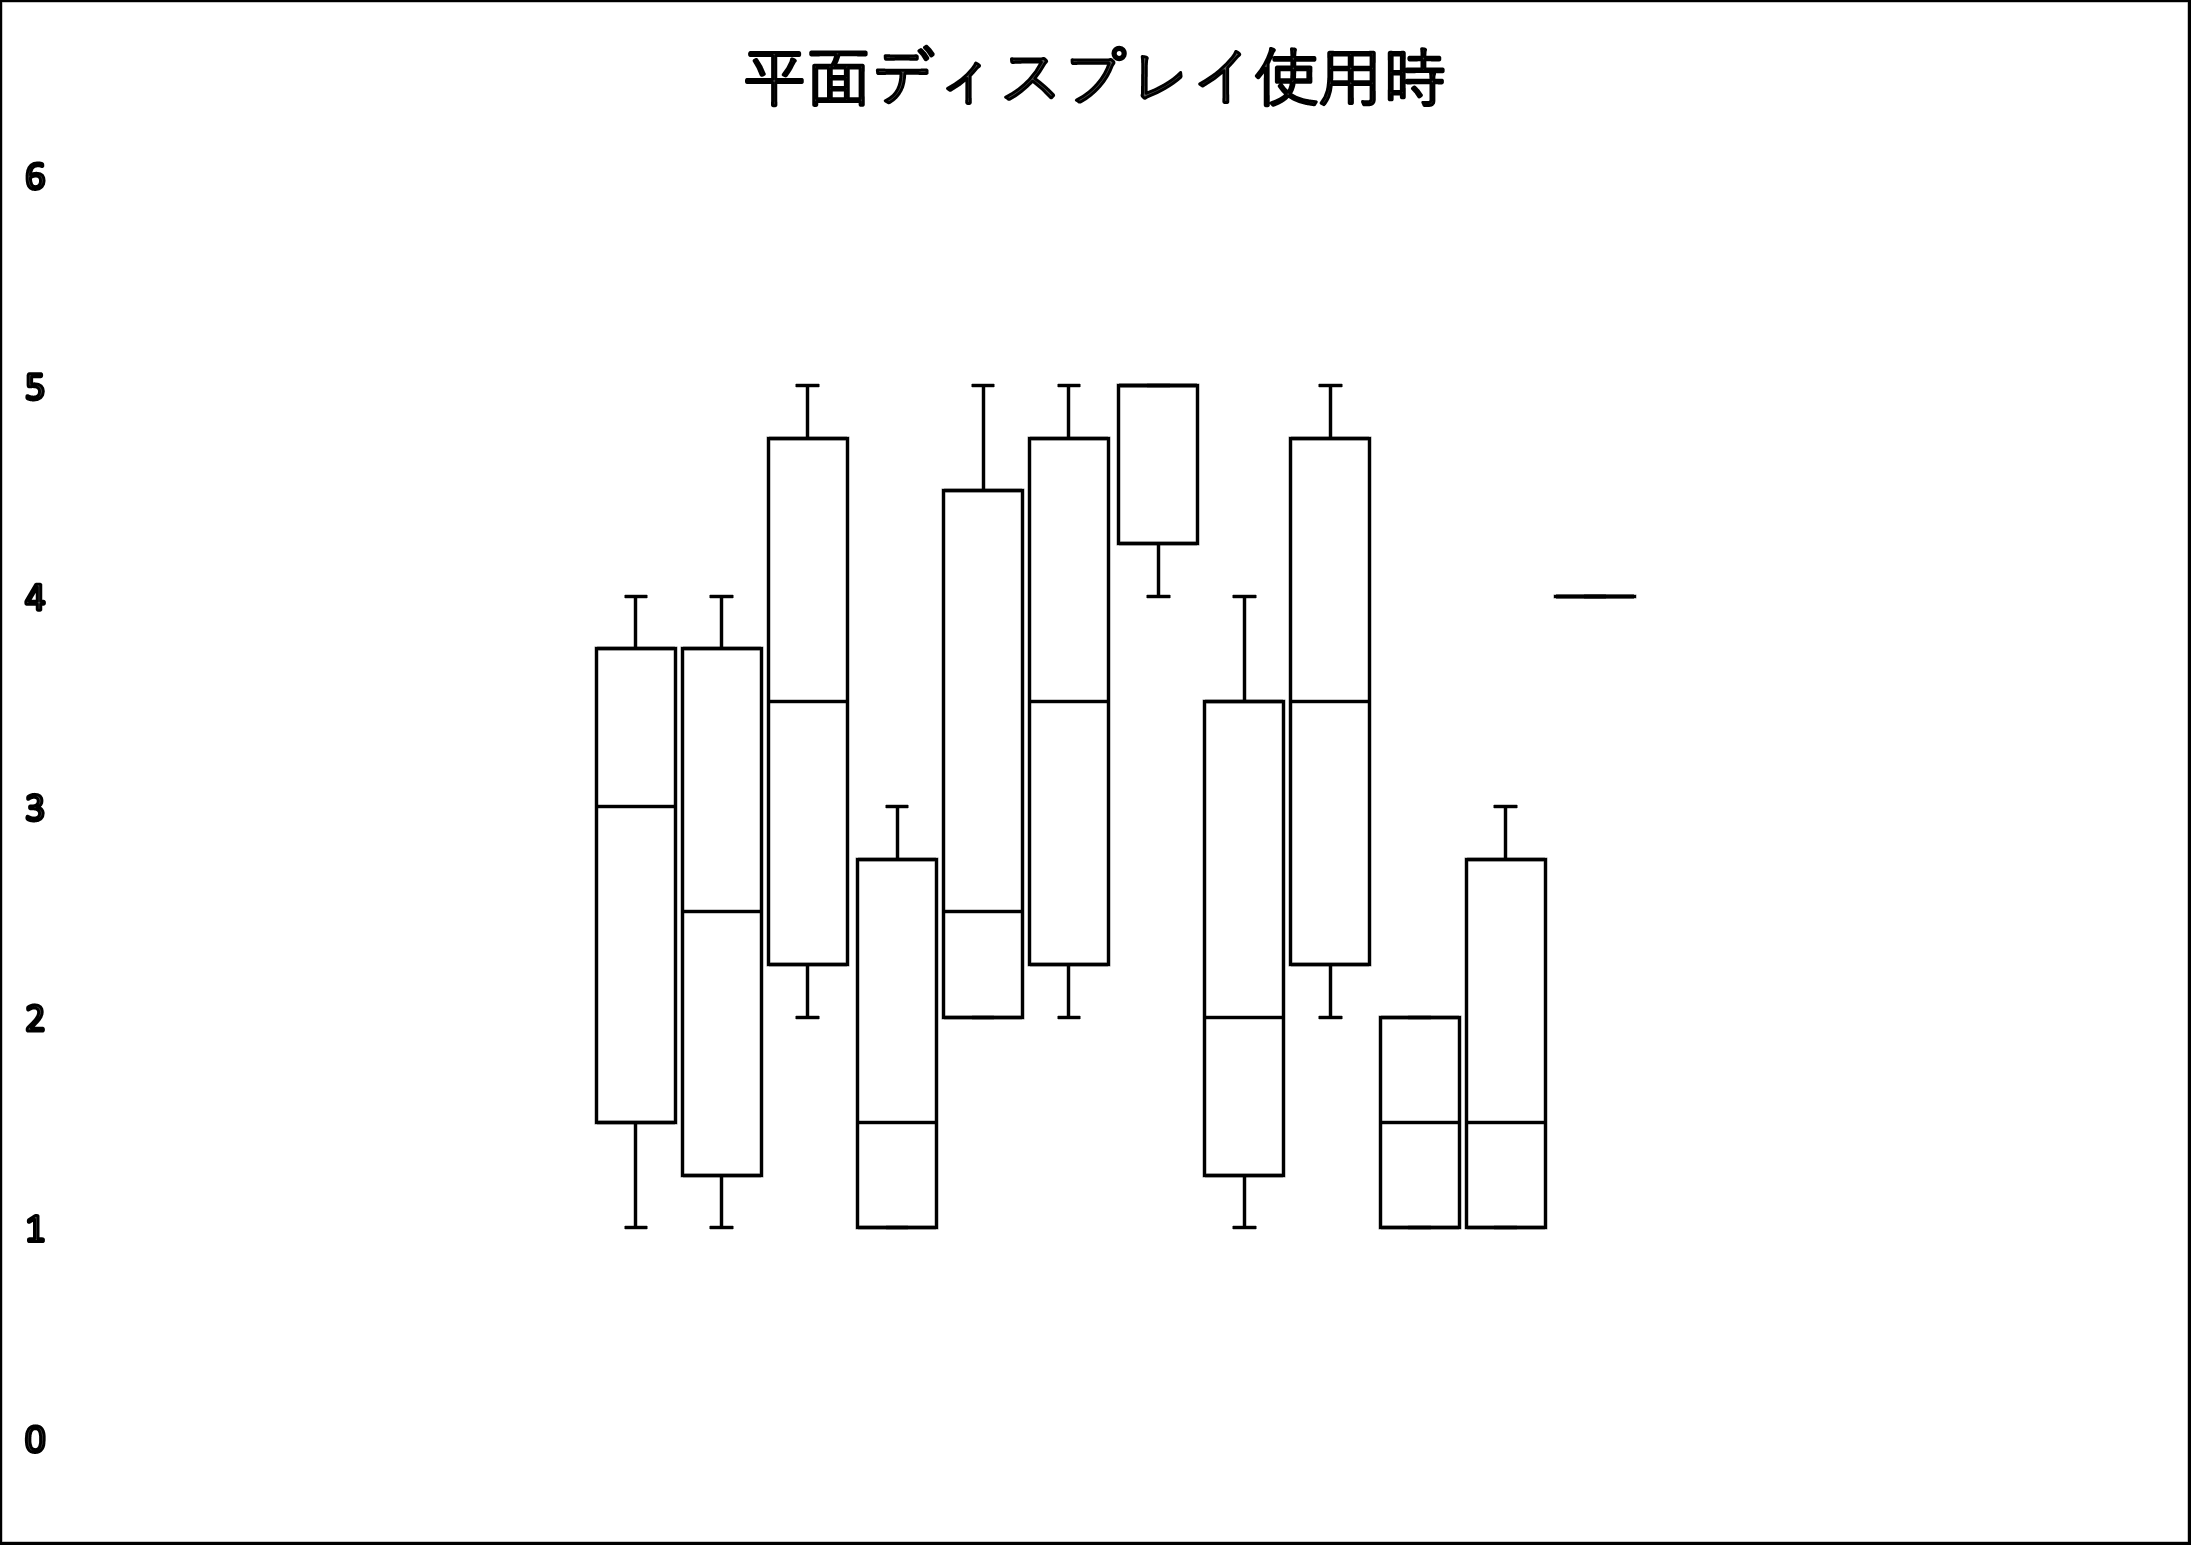
\includegraphics[scale=0.9]{fig/boxplot1.png}\label{boxplot1}
  \caption{平面ディスプレイ使用時の5段階評価項目結果}
  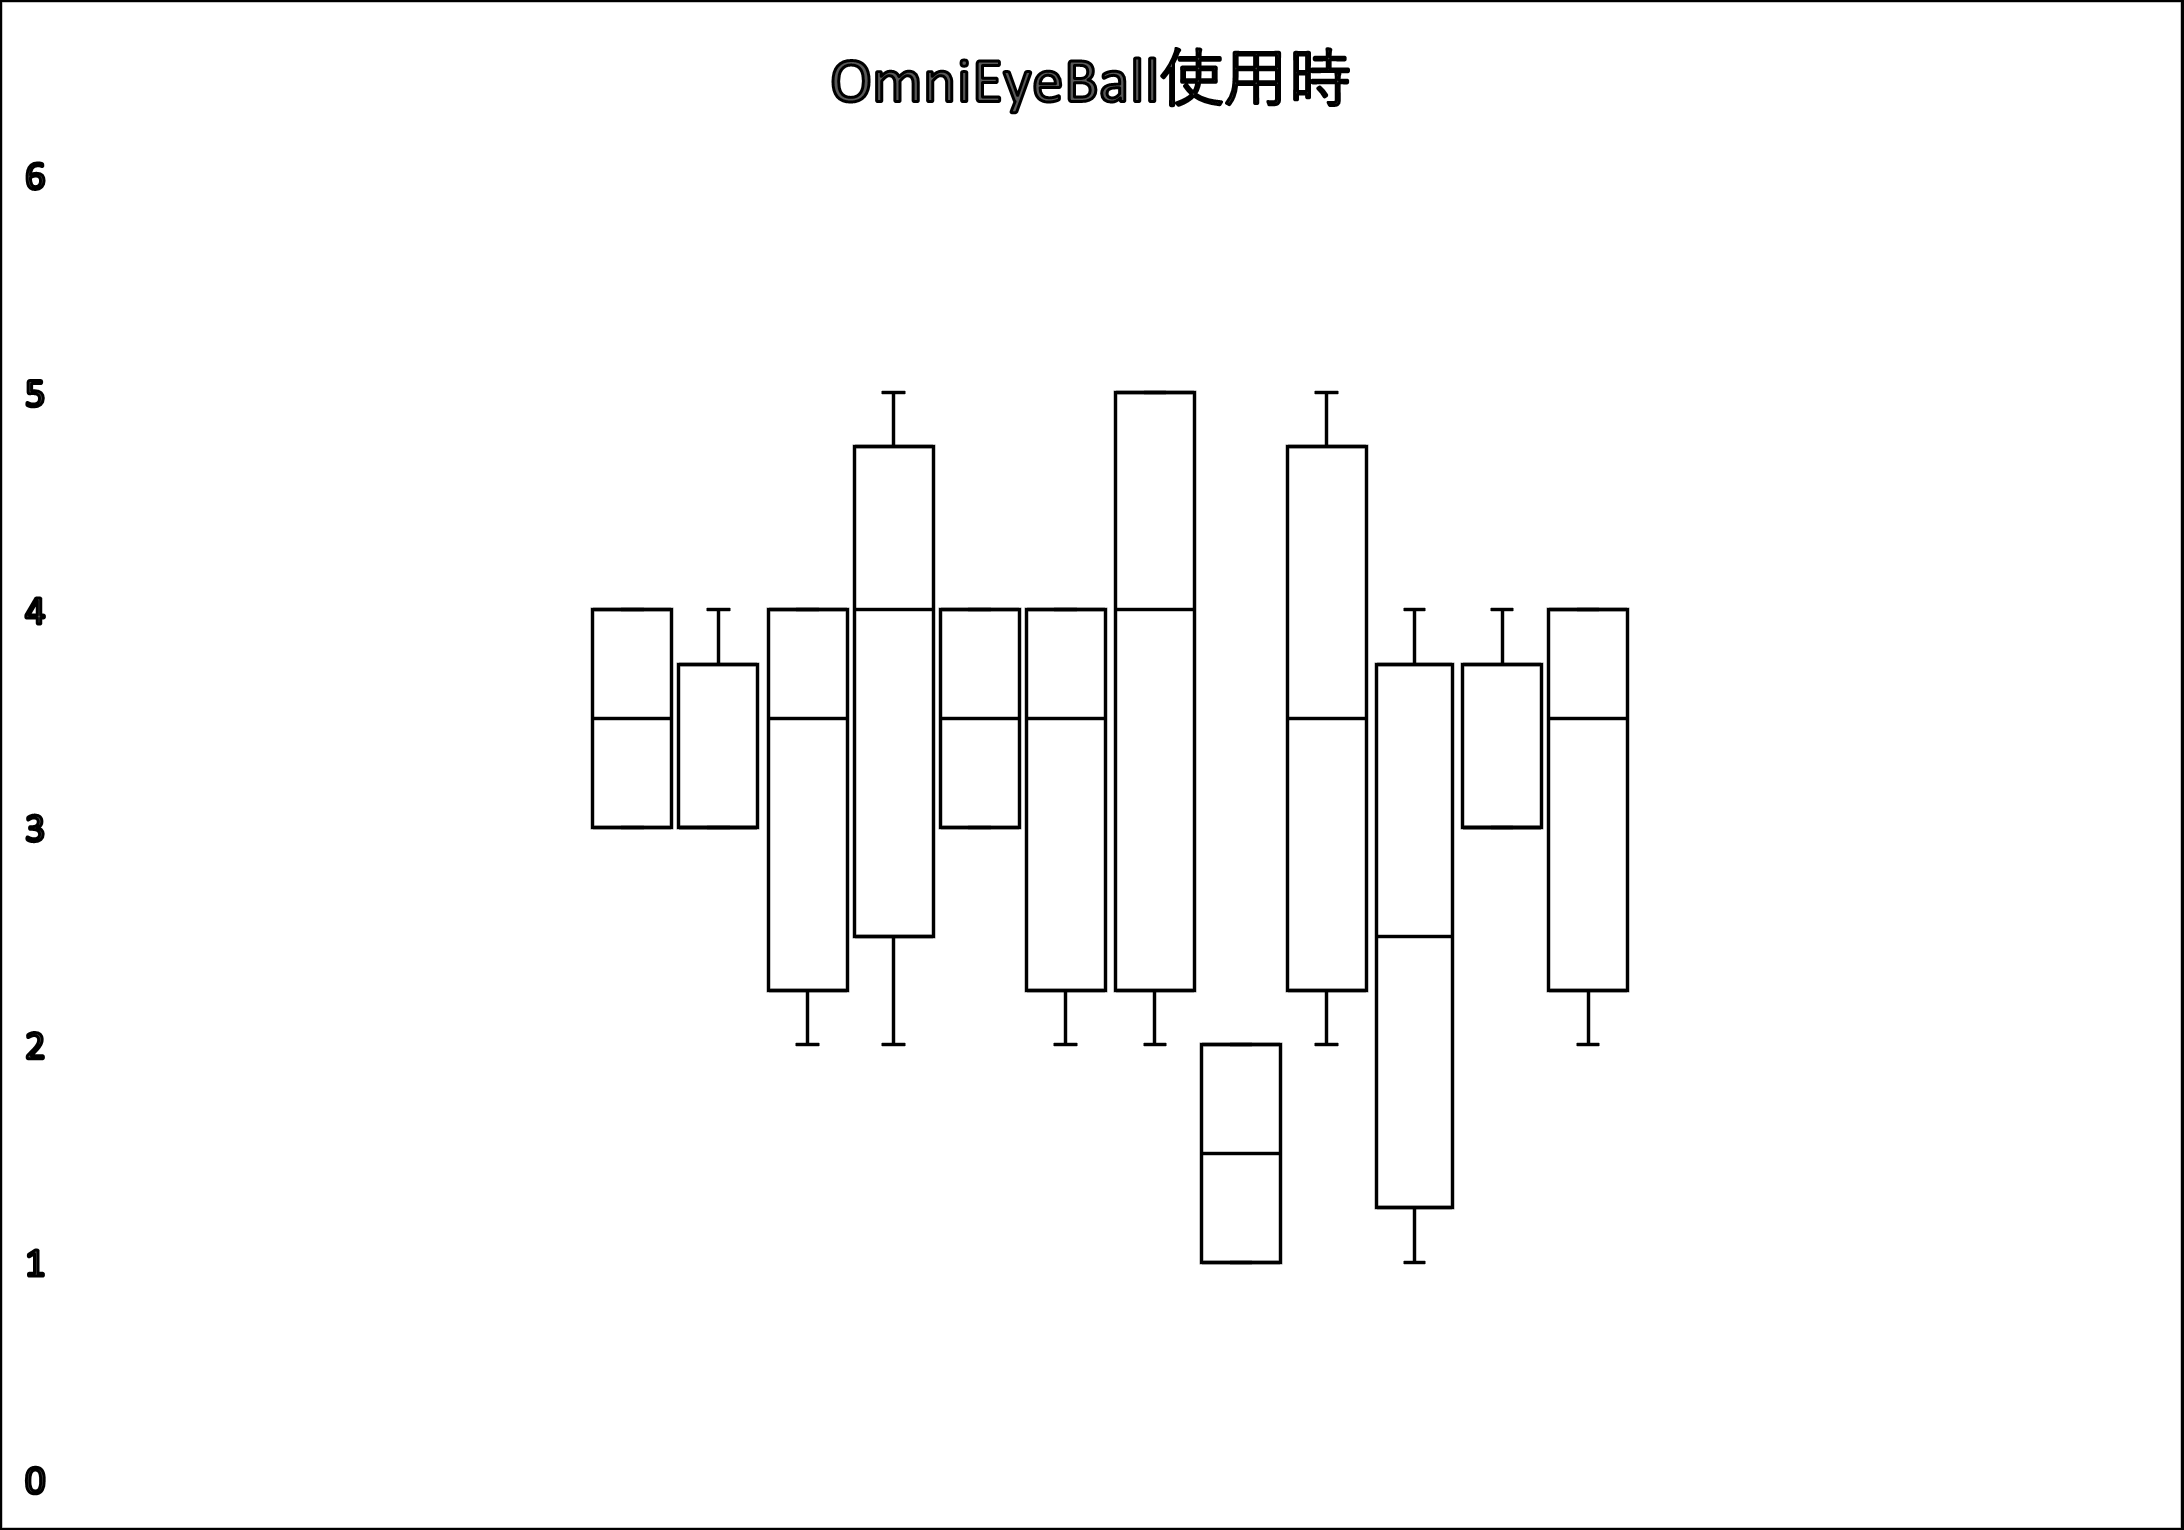
\includegraphics[scale=0.9]{fig/boxplot2.png}\label{boxplot2}
  \caption{OmniEyeBall使用時の5段階評価項目結果}
\end{figure}



\begin{table}[tp]
  \begin{center}
  \begin{tabular}{|c|c|c|}
  \hline
       & 平面時  & OEB時 \\ \hline
  質問1  & 2.75 & 3.5  \\ \hline
  質問2  & 2.5  & 3.25 \\ \hline
  質問3  & 3.5  & 3.25 \\ \hline
  質問4  & 1.75 & 3.75 \\ \hline
  質問5  & 3    & 3.5  \\ \hline
  質問6  & 3.5  & 3.25 \\ \hline
  質問7  & 4.75 & 3.75 \\ \hline
  質問8  & 2.25 & 1.5  \\ \hline
  質問9  & 3.5  & 3.5  \\ \hline
  質問10 & 1.5  & 2.5  \\ \hline
  質問11 & 1.75 & 3.25 \\ \hline
  質問12 & 4    & 3.25 \\ \hline
  \end{tabular}\label{ave}
  \caption{各質問の4人の平均値}
\end{center}
  \end{table}

記述式項目については5-5節にて言及する.

また,平面ディスプレイを使用したケースとOmniEyeBallを使用したケースの
どちらが好ましいかを問う質問では,前者が好ましいと答えた人数は1人,
後者が好ましいと答えた人数は3人であった.